\documentclass[a4paper,10pt]{article}
\usepackage[utf8]{inputenc}
\usepackage[MeX]{polski}
\usepackage{tikz}
\usepackage{url}
\usepackage{fullpage}
\usepackage{titlesec}

\title{Projekt MED-P3, algorytm GRM. Raport. \\ \small{Przedmiot: Metody eksploracji danych w odkrywaniu wiedzy.}}
\author{Michał Aniserowicz, Jakub Turek}
\date{}

\begin{document}

\maketitle

\section{Opis zadania} \label{sec:task_desc}
Celem projektu jest zaimplementowanie algorytmu wyznaczania reguł decyzyjnych o minimalnych poprzednikach, które są częstymi generatorami.
Algorytm ten jest modyfikacją algorytmu odkrywania częstych generatorów (GRM), opisanego w~\cite{grm}.



\section{Założenia} \label{sec:assumptions}
Projekt zrealizowano w oparciu o następujące założenia:

 \subsection{Niefunkcjonalne:}
  \begin{enumerate}
   \item Użyty język programowania; platforma: C\#; .NET Framework 3.5.
   \item Obsługiwane systemy operacyjne: kompatybilne z .NET Framework 3.5\footnote{Lista systemów kompatybilnych z .NET Framework 3.5 dostępna jest pod adresem: \emph{http://msdn.microsoft.com/en-us/library/vstudio/bb882520\%28v=vs.90\%29.aspx}, sekcja ``Supported Operating Systems''.} (aplikację testowano na systemie Microsoft Windows 7 Ultimate).
   \item Rodzaj aplikacji: aplikacja konsolowa uruchamiana z wiersza poleceń.
 \end{enumerate}


 \subsection{Funkcjonalne:}
  \begin{enumerate}
   \item Aplikacja pobiera dane z pliku (patrz sekcja~\ref{sec:input:file}).
   \item Aplikacja zwraca wynik działania w dwóch formatach: ``przyjaznym dla człowieka'' i ``excelowym'' (patrz sekcja~\ref{sec:output}).
   \item Aplikacja pozwala mierzyć czas wykonania poszczególnych kroków algorytmu.
  \end{enumerate}


 \subsection{Dotyczące danych wejściowych:} \label{sec:assumptions:input}
  \begin{enumerate}
   \item Dane wejściowe zawierają jedynie wartości atrybutów transakcji i ewentualnie nazwy atrybutów transakcji.
   \item Wartości atrybutów w pliku wejściowym są oddzielone przecinkami.
   \item Każda transakcja ma przypisaną decyzję.
   \item Brakujące wartości atrybutów (tzn. wartości nieznane bądź nieustalone) są oznaczone jako wartości puste lub złożone z białych znaków.
  \end{enumerate}



\section{Dane wejściowe} \label{sec:input}
Aplikacja będąca wynikiem projektu przyjmuje jednocześnie dwa rodzaje danych wejściowych:

\begin{itemize}
 \item plik zawierający dane transakcji,
 \item parametry podane przez użytkownika w wierszu poleceń.
\end{itemize}

 \subsection{Plik wejściowy} \label{sec:input:file}
 Plik wejściowy powinien zawierać kolejne wartości atrybutów transakcji według reguł przedstawionych w sekcji~\ref{sec:assumptions:input}.
 Przykładowy format pliku wejściowego:
 
\begin{verbatim}
a,b,c,d,e, ,g, ,+
a,b,c,d,e,f, , ,+
a,b,c,d,e, , ,h,+
a,b, ,d,e, , , ,+
a, ,c,d,e, , ,h,-
 ,b,c, ,e, , , ,-
\end{verbatim}

 Opcjonalnie, pierwszy wiersz pliku wejściowego może zawierać nazwy atrybutów transakcji (nagłówki), na przykład:

\begin{verbatim}
Attr A,Attr B,Attr C,Attr D,Attr E,Attr F,Attr G,Attr H,Decision
a,b,c,d,e, ,g, ,+
 ,b,c, ,e, , , ,-
\end{verbatim}

 Jeden z atrybutów transakcji musi reprezentować przypisaną jej decyzję.
 Domyślnie, aplikacja uznaje ostatni atrybut transakcji za ``decyzyjny'' - użytkownik może jednak samodzielnie wskazać odpowiedni atrybut (patrz sekcja~\ref{sec:input:cmd}).
 
 
 \subsection{Parametry wiersza poleceń} \label{sec:input:cmd}
 Aplikacja przyjmuje następujące parametry:
 
 \begin{itemize}
  \item \verb+--help+ - Powoduje wyświetlenie informacji o dostępnych parametrach i wyjście z programu.
  \item \verb+-f, --file=VALUE+ - Ścieżka do pliku wejściowego. Parametr wymagany.
  \item \verb+--sup, --minSup=VALUE+ - Próg (bezwzględny) wsparcia - wykryte zostaną reguły decyzyjne o poprzednikach cechujących się wsparciem większym \textbf{lub równym} progowi wsparcia. Parametr wymagany.
  \item \verb+-h, --headers+ - Flaga oznaczająca, że plik wejściowy zawiera nagłówki atrybutów. Parametr opcjonalny.
  \item \verb+--dec, --decAttr=VALUE+ - Pozycja atrybutu zawierającego wartości decyzji (\verb+1+ - pierwszy atrybut, \verb+2+ - drugi atrybut itd.). Parametr opcjonalny (jeśli nie zostanie podany, ostatni atrybut zostanie uznany za decyzyjny).
  \item \verb+--sort=VALUE+ - strategia sortowania elementów (patrz sekcja~\ref{sec:impl:sort}). Parametr opcjonalny.
  Dopuszczalne wartości:
  \begin{itemize}
   \item \verb+AscendingSupport+ (lub \verb+0+; wartość domyślna),
   \item \verb+DescendingSupport+ (lub \verb+1+),
   \item \verb+Lexicographical+ (lub \verb+2+).
  \end{itemize}
 
  \item \verb+--store=VALUE+ - strategia przechowywania identyfikatorów transakcji (patrz sekcja~\ref{sec:impl:store}). Parametr opcjonalny.
  Dopuszczalne wartości:
  \begin{itemize}
   \item \verb+TIDSets+ (lub \verb+0+; wartość domyślna),
   \item \verb+DiffSets+ (lub \verb+1+).
  \end{itemize}
  
  \item \verb+--supgen=VALUE+ - Strategia przechowywania generatorów decyzji, a także wykrywania i usuwania ich nadgeneratorów (patrz sekcja~\ref{sec:impl:supgen}). Parametr opcjonalny.
  Dopuszczalne wartości:
  \begin{itemize}
   \item \verb+InvertedLists+ (lub \verb+0+; wartość domyślna),
   \item \verb+BruteForce+ (lub \verb+1+).
  \end{itemize}
  
  \item \verb+--track=VALUE+ - Poziom monitorowania wydajności programu (patrz sekcja~\ref{sec:impl:track}). Parametr opcjonalny.
  \begin{itemize}
   \item \verb+NoTracking+ (lub \verb+0+),
   \item \verb+Task+ (lub \verb+1+; wartość domyślna).
   \item \verb+Steps+ (lub \verb+2+).
   \item \verb+Substeps+ (lub \verb+3+; Uwaga: może powodować znaczący spadek ogólnej wydajności programu).
  \end{itemize}
  
  \item \verb+-o, --output=VALUE+ - Ścieżka plików wyjściowych. Parametr opcjonalny. Poprawna wartość jest ścieżką pliku z pominięciem jego rozszerzenia (np. \emph{wyniki/wynik}. Wartość domyślna: \emph{[ścieżka pliku wejściowego]\_rules}.
 \end{itemize}



\section{Dane wyjściowe} \label{sec:output}
Na wyjście aplikacji składają się trzy rodzaje danych:

\begin{itemize}
 \item komunikaty diagnostyczne wypisywane na standardowe wyjście,
 \item plik zawierący znalezione reguły decyzyjne w formacie czytelnym dla człowieka,
 \item plik zawierący znalezione reguły decyzyjne w formacie przystosowanym do dalszej obróbki.
\end{itemize}

 \subsection{Plik czytelny dla człowieka} \label{sec:output:human}
 Plik w formacie czytelnym dla człowieka zawiera listy generatorów dla każdej decyzji.
 Pojedynczy generator jest przedstawiony jako lista wartości atrybutów wraz z ich nazwami.
 Przykład:
 
\begin{verbatim}
====================
Decision: '+':
--------------------
Attr A (a), Attr B (b)
Attr B (b), Attr D (d)
\end{verbatim}

 Plik ten jest zapisywany pod ścieżką \emph{[plik].txt}, gdzie \emph{[plik]} to wartość parametru \verb+output+ (patrz sekcja~\ref{sec:input:cmd}).

 
 \subsection{Plik przystosowany do dalszej obróbki} \label{sec:output:csv}
 Plik w formacie czytelnym dla człowieka zawiera listę generatrów wraz generowanymi przez nie decyzjami.
 Pojedynczy generator jest przedstawiony jako lista wartości oddzielonych średnikami\footnote{Patrz http://pl.wikipedia.org/wiki/CSV\_(format\_pliku). W omawianej aplikacji zamiast przecinków użyto średników, aby plik wyjściowy mógł być odczytany przez program Microsoft Excel.}, z uwzględnieniem atrybutów niewystępujących w generatorze.
 Przykład:
 
\begin{verbatim}
Attr A;Attr B;Attr C;Attr D;Attr E;Attr F;Attr G;Attr H;Decision
a;b;;;;;;;+
;b;;d;;;;;+
\end{verbatim}
 
 Plik ten jest zapisywany pod ścieżką \emph{[plik].csv}, gdzie \emph{[plik]} to wartość parametru \verb+output+ (patrz sekcja~\ref{sec:input:cmd}).



\section{Architektura aplikacji} \label{sec:arch}
Aplikacja składa się z następujących modułów:

\begin{itemize}
 \item \verb+GRM.Logic+ - zawiera implementację zmodyfikowanego algorytmu GRM,
 \item \verb+GRM.Logic.UnitTests+ - zawiera testy jednostkowe modułu \verb+GRM.Logic+,
 \item \verb+GRM.Logic.PerformanceTests+ - zawiera testy wydajnościowe modułu \verb+GRM.Logic+, 
 \item \verb+GRM.Presentation+ - aplikacja konsolowa przetwarzająca argumenty wiersza poleceń i wywołująca algorytm GRM.
\end{itemize}


 \subsection{Moduł GRM.Logic}
 Moduł \verb+GRM.Logic+ jest głównym modułem aplikacji.
 Zawiera implementację zmodyfikowanego algorytmu GRM.
 Jego diagram klas został przedstawiony na Rysunku~\ref{fig:diag:log:class}.

 \begin{figure}[!ht]
  \begin{center}
   \scalebox{0.42}
   {
    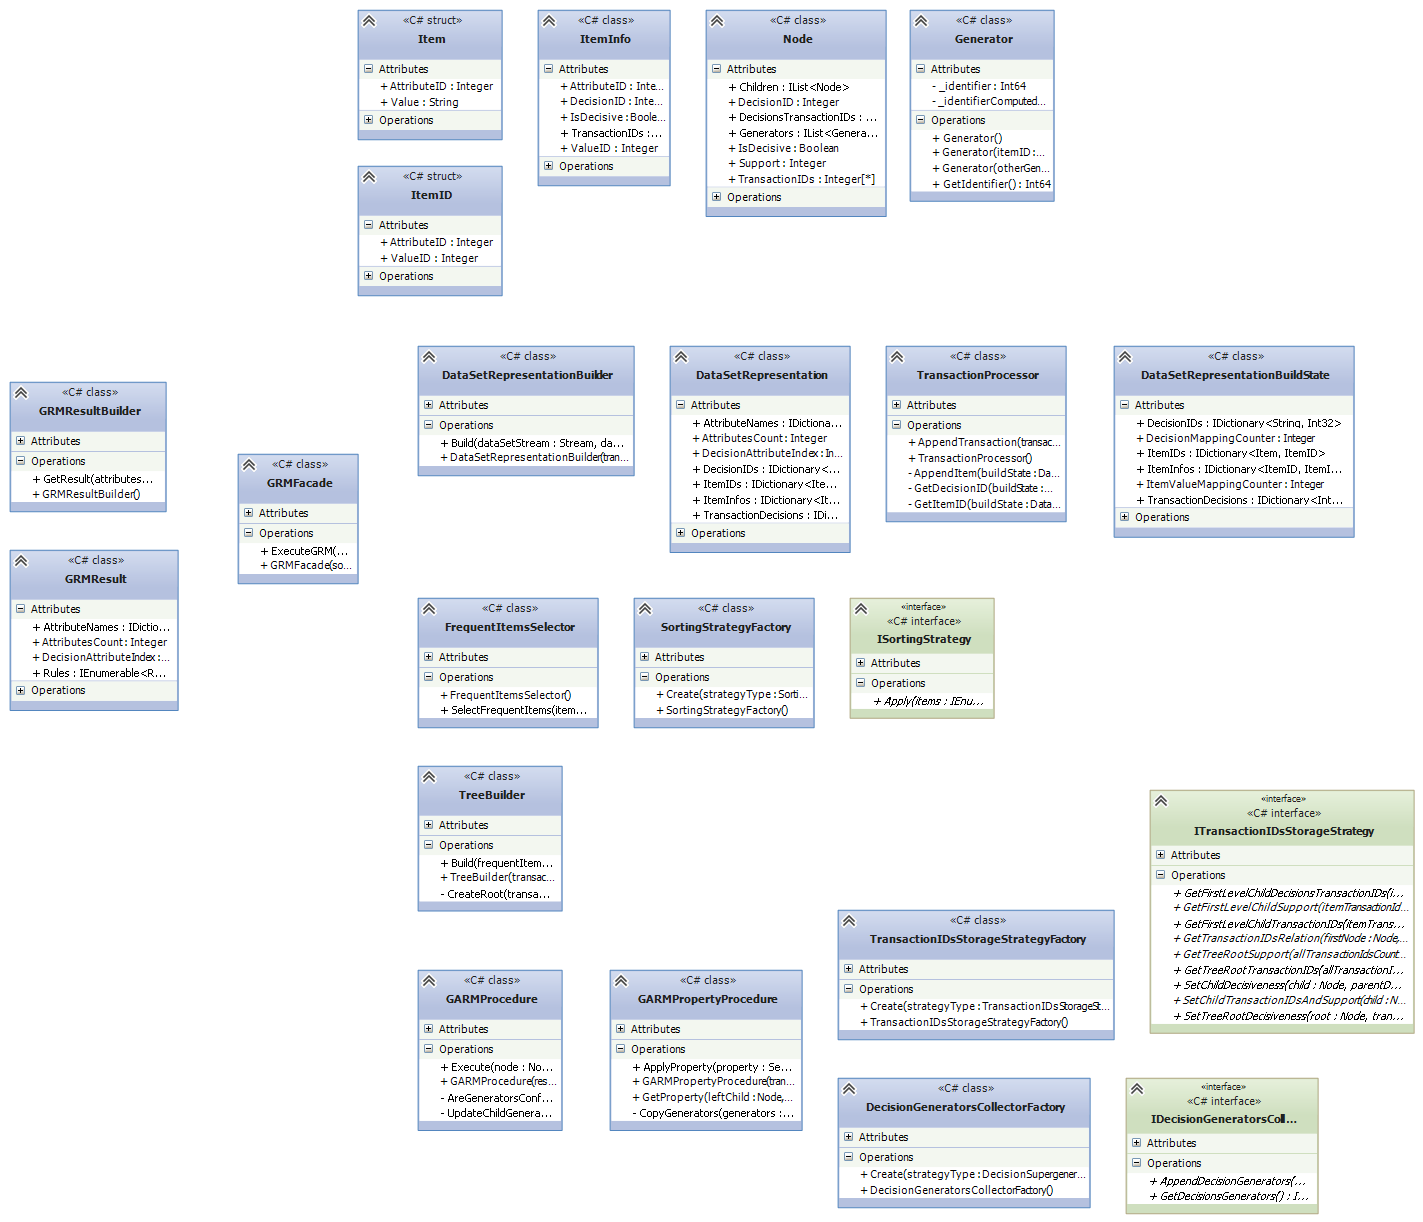
\includegraphics{../diagrams/Logic_class_diagram.png}
   }
  \end{center}
  \caption{
   Uproszczony diagram klas modułu GRM.Logic.
  }
  \label{fig:diag:log:class}
 \end{figure}
  
 Punktem wejścia modułu jest klasa \verb+GRMFacade+.
 Zleca ona wykonanie kolejnych kroków algorytmu.
 Diagram jej zależności przedstawia Rysunek~\ref{fig:diag:log:Facade}.
 
 \begin{figure}[!ht]
  \begin{center}
   \scalebox{0.7}
   {
    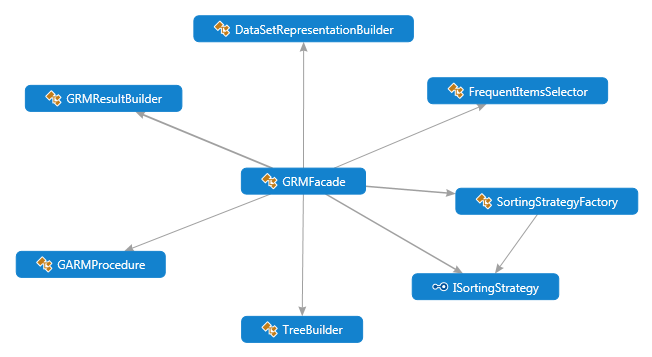
\includegraphics{../diagrams/GRMFacade_dependency_diagram.png}
   }
  \end{center}
  \caption{
   Uproszczony diagram zależności fasady modułu GRM.Logic.
  }
  \label{fig:diag:log:Facade}
 \end{figure}
 
 Poszczególne kroki algorytmu zaimplementowane są w dwóch komponentach:
 
 \begin{itemize}
  \item GRM.Logic.DataSetProcessing,
  \item GRM.Logic.GRMAlgorithm.
 \end{itemize}

 
  \subsubsection{Komponent GRM.Logic.DataSetProcessing}
  Zadaniem komponentu \verb+GRM.Logic.DataSetProcessing+ jest odczytanie pliku wejściowego i zbudowanie reprezentacji zbioru danych przeznaczonej do dalszego przetwarzania.
  
  Diagram zależności tego komponentu został przedstawiony na Rysunku~\ref{fig:diag:log:DataSetProcessing}.
  
  \begin{figure}[!ht]
   \begin{center}
    \scalebox{0.7}
    {
     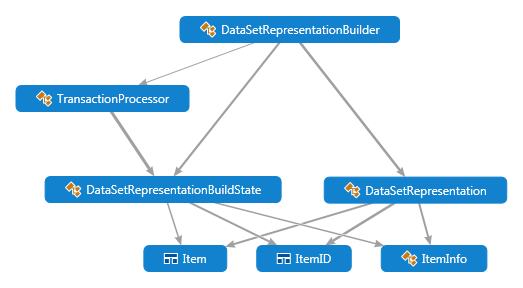
\includegraphics{../diagrams/DataSetProcessing_dependency_diagram.png}
    }
   \end{center}
   \caption{
    Uproszczony diagram zależności komponentu GRM.Logic.DataSetProcessing.
   }
   \label{fig:diag:log:DataSetProcessing}
  \end{figure}
 
  \subsubsection{Komponent GRM.Logic.GRMAlgorithm}
  Komponent GRM.Logic.GRMAlgorithm implementuje zmodyfikowany algorytm GRM.
  Jego diagram zależności przedstawia Rysunek~\ref{fig:diag:log:GRMAlgorithm}.
  
  \begin{figure}[!ht]
   \begin{center}
    \scalebox{0.7}
    {
     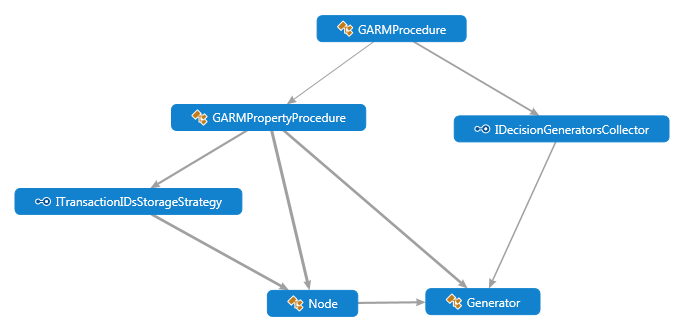
\includegraphics{../diagrams/GRMAlgorithm_dependency_diagram.png}
    }
   \end{center}
   \caption{
    Uproszczony diagram zależności komponentu GRM.Logic.GRMAlgorithm.
   }
   \label{fig:diag:log:GRMAlgorithm}
  \end{figure}


 \subsection{Moduł GRM.Presentation}
 Moduł \verb+GRM.Presentation+ odpowiada za komunikację z użytkownikiem aplikacji i zlecenie wykonania algorytmu GRM.
 Jego diagram klas przedstawia Rysunek~\ref{fig:diag:log:class}.
 
 \begin{figure}[!ht]
  \begin{center}
   \scalebox{0.55}
   {
    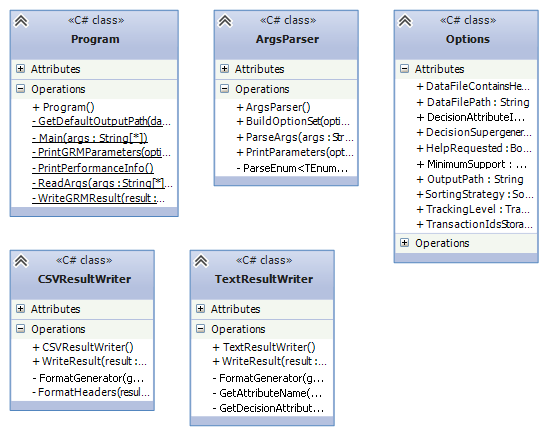
\includegraphics{../diagrams/Presentation_class_diagram.png}
   }
  \end{center}
  \caption{
   Diagram klas modułu GRM.Presentation.
  }
  \label{fig:diag:pres:class}
 \end{figure}
 
 Klasa \verb+Program+ zawiera główną metodę programu - \verb+Main+. 
 Jej działanie przebiega następująco:
 
 \begin{enumerate}
  \item Odczytanie parametrów wiersza poleceń (klasa \verb+ArgsParser+).
  Błędne parametry skutkują wypisaniem komuniaktu o błędzie i wyjściem z aplikacji.
  \item Przekazanie sterowania modułowi \verb+GRM.Logic+ (klasie \verb+GRMFacade+).
  \item Odebranie wyniku działania algorytmu GRM (\verb+GRMResult+) od klasy \verb+GRMFacade+.
  \item Wypisanie zebranych danych o czasach trwania kolejnych kroków algorytmu (patrz sekcja~\ref{sec:impl:track}).
  \item Zapisanie wyniku działania algorytmu do pliku wyjściowego w formacie czytelnym dla człowieka (klasa \verb+TextResultWriter+).
  \item Zapisanie wyniku działania algorytmu do pliku wyjściowego w formacie przystosowanym do dalszej obróbki (klasa \verb+CSVResultWriter+).
 \end{enumerate}
 
 Opisane zachowanie obrazuje diagram zależności pokazany na Rysunku~\ref{fig:diag:pres:dep}.
 
 \begin{figure}[!ht]
  \begin{center}
   \scalebox{0.7}
   {
    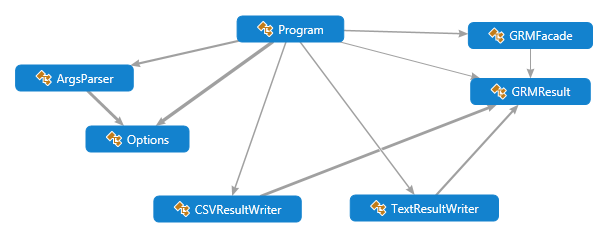
\includegraphics{../diagrams/Presentation_dependency_diagram.png}
   }
  \end{center}
  \caption{
   Diagram zależności modułu GRM.Presentation.
   Klasy GRMFacade i GRMResult należą do modułu GRM.Logic.
  }
  \label{fig:diag:pres:dep}
 \end{figure}


\section{Implementacja} \label{sec:impl}
Najważniejsze aspekty implementacyjne opisywanej aplikacji:

 \subsection{Kroki algorytmu}
 Działanie modułu \verb+GRM.Logic+ przebiega w następujących krokach:\\
 \emph{[W nawiasach kwadratowych podano nazwę klasy wykonującej dany krok.]}
 
 \begin{enumerate}
  \item $[$\verb+DataSetRepresentationBuilder+$]$ Odczytanie pliku wejściowego i budowa reprezentacji zbioru danych:
   \begin{enumerate}
    \item określenie liczby atrybutów i odczytanie ich nagłówków (jeśli dostępne);
    \item dla każdego z wierszy reprezentujących transakcje:
     \begin{enumerate}
      \item $[$\verb+TransactionProcessor+$]$ nadanie identyfikatora transakcji,
      \item $[$\verb+TransactionProcessor+$]$ dla każdego elementu transakcji:
       \begin{enumerate}
        \item nadanie identyfikatora elementu (jeśli element o tej wartości jeszcze nie wystąpił),
        \item aktualizacja danych elementu (zbioru transakcji, w których występuje i decyzyjności);
       \end{enumerate}
     \end{enumerate}
    \item zwrócenie gotowej reprezentacji danych (\verb+DataSetRepresentation+).
   \end{enumerate}

  \item $[$\verb+FrequentItemsSelector+$]$ Wybór elementów częstych.
  
  \item $[$\verb+ISortingStrategy+$]$ Posortowanie elementów częstych.
  
  \item $[$\verb+TreeBuilder+$]$ Budowa drzewa zbiorów (drzewa DZ~\cite{grm}):
   \begin{enumerate}
    \item utworzenie korzenia drzewa:
     \begin{enumerate}
      \item $[$\verb+ITransactionIDsStorageStrategy+$]$ wyznaczenie zbioru identyfikatorów transakcji korzenia;
     \end{enumerate} 
    \item utworzenie pierwszego poziomu węzłów drzewa - dla każdego z elementów częstych:
     \begin{enumerate}
      \item ustawienie elementu jako generatora węzła,
      \item $[$\verb+ITransactionIDsStorageStrategy+$]$ wyznaczenie zbioru identyfikatorów transakcji węzła oraz jego wsparcia i decyzyjności;
     \end{enumerate}
    \item zwrócenie korzenia drzewa zbiorów (\verb+Node+).
   \end{enumerate}

  \item $[$\verb+GARMProcedure+$]$ Wywołanie procedury GARM~\cite{grm}.
  
  \item $[$\verb+GRMResultBuilder+$]$ Budowa i zwrócenie wyniku (\verb+GRMResult+).
 \end{enumerate}

 
 \subsection{Strategie sortowania elementów} \label{sec:impl:sort}
 Zaimplementowano następujące strategie sortowania elementów w drzewie zbiorów:
 
 \begin{itemize}
  \item \verb+AscendingSupport+ (klasa \verb+AscendingSupportSortingStrategy+) - sortowanie rosnące według wsparć elementów,
  \item \verb+DescendingSupport+ (klasa \verb+DescendingSupportSortingStrategy+) - sortowanie malejące według wsparć elementów,
  \item \verb+Lexicographical+ (klasa \verb+LexicographicalSortingStrategy+) - sortowanie leksykograficzne. tzn. według numerów atrybutów elementów (dla dwóch wartości tego samego atrybutu, pierwsza będzie ta, która wcześniej wystąpiła w zbiorze danych wejściowych).
 \end{itemize}
 
 Strategie sortowania dostarcza fabryka \verb+SortingStrategyFactory+, tworząca strategie odpowiadające zadanym wartościom wyliczenia \verb+SortingStrategyType+.

 
 \subsection{Strategie przechowywania identyfikatorów transakcji} \label{sec:impl:store}
 Zaimplementowano następujące strategie przechowywania identyfikatorów transakcji:
 
 \begin{itemize}
  \item \verb+TIDSets+~\cite{charm} (klasa \verb+TIDSetsStorageStrategy+),
  \item \verb+DiffSets+~\cite{grm} (klasa \verb+DiffSetsStorageStrategy+).
 \end{itemize}

 Strategie przechowywania dostarcza fabryka \verb+TransactionIDsStorageStrategyFactory+, tworząca strategie odpowiadające zadanym wartościom wyliczenia \verb+TransactionIDsStorageStrategyType+.

 
 \subsection{Strategie przechowywania generatorów decyzji} \label{sec:impl:supgen}
 Zaimplementowano następujące strategie przechowywania generatorów decyzji, a także wykrywania i usuwania ich nadgeneratorów:
 
 \begin{itemize}
  \item \verb+InvertedLists+ (klasa \verb+InvertedListsDecisionGeneratorsCollector+) - wykorzystuje koncepcję indeksu odwróconego\footnote{Patrz http://en.wikipedia.org/wiki/Inverted\_index.}, gdzie kluczem indeksu jest element, a wartością - lista generatorów, w których ten element występuje,
  \item \verb+BruteForce+ (klasa \verb+BruteForceDecisionGeneratorsCollector+) - przechowuje jedynie listę generatorów, nadgeneratory wykrywa porównując każdy element danego generatora z każdym elementem jego potencjalnego nadgeneratora.
 \end{itemize}
 
 Strategie dostarcza fabryka \verb+DecisionGeneratorsCollectorFactory+, tworząca strategie odpowiadające zadanym wartościom wyliczenia \verb+DecisionSupergeneratorsHandlingStrategyType+.
 
 
 \subsection{Monitorowanie wydajności programu} \label{sec:impl:track}
 Aplikacja udostępnia funkcjonalność mierzenia czasu wykonania poszczególnych kroków algorytmu.
 Zaimplementowano następujące rodzaje pomiaru:
 
 \begin{itemize}
  \item \verb+NoTracking+ (klasa \verb+EmptyProgressTracker+) - brak pomiaru wydajności,
  \item \verb+Task+ (klasa \verb+TaskProgressTracker+) - pomiar czasu trwania całego algorytmu,
  \item \verb+Steps+ (klasa \verb+StepProgressTracker+) - pomiar czasu trwania głównych kroków algorytmu (odczyt danych wejściowych, wykonanie procedury \emph{GARM} itd.),
  \item \verb+Substeps+ (klasa \verb+SubstepProgressTracker+) - pomiar czasu trwania mniejszych kroków algorytmu (budowanie słownika identyfikatorów decyzji, wykonanie procedury \emph{GARM-Property} itd.). Uwaga: może powodować znaczący spadek ogólnej wydajności programu.
 \end{itemize}

 Obiekty monitorujące dostarcza fabryka \verb+ProgressTrackerFactory+, tworząca obiekty odpowiadające zadanym wartościom wyliczenia \verb+TrackingLevel+.

 \subsection{Zabiegi optymalizacyjne}
 \begin{itemize}
  \item Aby zminimalizować czas odczytu danych wejściowych, plik wejściowy jest odczytywany jednokrotnie, wiersz po wierszu.
  \item Aby zminimalizować czas trwania porównań, wszystkie wartości atrybutów otrzymują identyfikatory liczbowe.
  \item Aby zminimalizować czas operacji (np. przecięcia, różnicy) na zbiorach identyfikatorów transakcji, identyfikatory te są przechowywane w ustalonym (rosnącym) porządku.
  \item Aby możliwie wcześnie ``odciąć'' gałęzie drzewa, które nie prowadzą do znalezienia generatorów decyzji:
   \begin{itemize}
    \item jeśli dwa węzły zawierają różne wartości tego samego atrybutu, to nie są ``parowane'' (tzn. poddawane procedurze \emph{GARM-Property}) - przecięcie zbiorów identyfikatorów transakcji, w których występują jest puste, a zatem ich potencjalne dziecko nie może generować żadnej decyzji;
    \item jeśli dany węzeł jest ``decyzyjny'' (tzn. generuje decyzję), to nie jest dalej rozwijany - generatory jego potencjalnych dzieci byłyby nadgeneratorami jego generatora.
   \end{itemize}
  \item Jako że generator dowolnej decyzji $D_1$ nie może być nadgeneratorem żadnego generatora decyzji $D_2$ ($D_1 \ne D_2$), strategie przechowywania generatorów decyzji (patrz sekcja~\ref{sec:impl:supgen}) przechowują generatory w słownikach, których kluczami są identyfikatory decyzji, a wartościami - zbiory generatorów tych decyzji.
  Pozwala to zminimalizować rozmiary porównywanych zbiorów generatorów.
  \item Granica GBd~\cite{grm} nie jest tworzona i aktualizowana, jako że nie jest wykorzystywana w poszukiwaniu reguł decyzyjnych.
 \end{itemize}

 \subsection{Zastosowane praktyki programistyczne}
 \begin{itemize}
  \item Test-Driven Development, TDD\footnote{Patrz http://pl.wikipedia.org/wiki/Test-driven\_development.} - najważniejsze funkcjonalności aplikacji powstały zgodnie z zachowaniem kolejności: testy jednostkowe $\rightarrow$ implementacja $\rightarrow$ refaktoryzacja.
  \item Dependency Injection\footnote{Patrz http://pl.wikipedia.org/wiki/Wstrzykiwanie\_zależności.} - obiekty klas tworzonych i wykorzystywanych przez klasę \verb+GRMFacade+ nie tworzą swoich zależności samodzielnie, a otrzymują je z zewnątrz.
  \item Wzorce projektowe:
   \begin{itemize}
    \item Fasada\footnote{Patrz http://pl.wikipedia.org/wiki/Fasada\_(wzorzec\_projektowy).} (klasa \verb+GRMFacade+),
    \item Budowniczy\footnote{Patrz http://pl.wikipedia.org/wiki/Budowniczy\_(wzorzec\_projektowy).} (para klas: \verb+DataSetRepresentationBuilder+ i \verb+TransactionProcessor+),
    \item Strategia\footnote{Patrz http://pl.wikipedia.org/wiki/Strategia\_(wzorzec\_projektowy).} (strategie opisane wyżej),
    \item Fabryka\footnote{Patrz http://pl.wikipedia.org/wiki/Fabryka\_abstrakcyjna\_(wzorzec\_projektowy).} (fabryki strategii opisane wyżej).
   \end{itemize}
 \end{itemize}
 
 
 \subsection{Wykorzystane biblioteki zewnętrzne}
 \begin{enumerate}
  \item \emph{NDesk.Options}\footnote{Patrz http://www.ndesk.org/Options.} - ułatwia przetwarzanie parametrów wiersza poleceń,
  \item \emph{xUnit.net}\footnote{Patrz http://xunit.codeplex.com/.} - umożliwia tworzenie automatycznych testów jednostkowych,
  \item \emph{moq}\footnote{Patrz https://github.com/Moq/moq4.} - wspiera tworzenie automatycznych testów jednostkowych.
 \end{enumerate}



\section{Analiza wydajności} \label{sec:anal}
wyniki jakosciowe i ilosciowe na (np. czas dzialania; liczba wzorcow)
uzyskane dla wiekszych (wielkich) zbiorow danych(np. z
http://archive.ics.uci.edu/ml/ or http://fimi.cs.helsinki.fi/data/ lub
uzgodnionych już wcześniej ze mna podczas konsultacji projektowych)


 \subsection{Wybór najlepszej strategii przechowywania generatorów}
 - uzasadnic supergenerators Inverted Lists
 
 \begin{center}
  \begin{tabular}{ | r || c | c | c | c | }
   \hline
   zbiór danych            & \multicolumn{2}{|c|}{\emph{nursey}} & \multicolumn{2}{|c|}{\emph{mushrooms}} \\
   \hline
   próg wsparcia; l. reguł & 1; 117           & 10; 60           & 5; 3239            & 20; 2635          \\
   \hline
   \verb+BruteForce+       & \textbf{1.687 s} & \textbf{0.917 s} & \textbf{21.5 s}    & \textbf{14.44 s}  \\
   \hline
   \verb+InvertedLists+    & \textbf{0,733 s} & \textbf{0,65 s}  & \textbf{6,14 s}    & \textbf{4,98 s}   \\
   \hline
   wzrost wydajności       & \textbf{57\%}    & \textbf{29\%}    & \textbf{71\%}      & \textbf{66\%}     \\
   \hline
  \end{tabular}
 \end{center}

 \subsection{Wybór najlepszej strategii sortowania elementów i przechowywania identyfikatorów transakcji}
 - ze storage TIDSets
 - ze sortowanie AscendingSupport
 - wykresy, wykresy
 - Załącznik~\ref{apx:results}
 
 
 \subsection{Wnioski}
 - ze dla duzej liczby atrybutow malo wydajny



\section{Przykład działania aplikacji} \label{sec:example}
Poniżej przedstawiono przykład działania programu dla niewielkiego zbioru danych\footnote{Zbiór danych pochodzi z \cite{grm}, został on jedynie uzupełniony o decyzje przypisane transakcjom.}:

 \subsection{Plik wejściowy}
 Załóżmy, że plik wejściowy został nazwany \verb+input.data+.
 Zawartość pliku:

\begin{verbatim}
Attr A,Attr B,Attr C,Attr D,Attr E,Attr F,Attr G,Attr H,Decision
a,b,c,d,e, ,g, ,+
a,b,c,d,e,f, , ,+
a,b,c,d,e, , ,h,+
a,b, ,d,e, , , ,+
a, ,c,d,e, , ,h,-
 ,b,c, ,e, , , ,-
\end{verbatim}


 \subsection{Parametry wiersza poleceń}
 Aplikacja zostaje uruchomiona z następującymi parametrami:
 
\begin{verbatim}
GRM.exe -f input.data -h --sup 3 --track 3
\end{verbatim}


 \subsection{Komunikaty wypisane na konsoli}
 Na konsoli wypisane zostają następujące komunikaty:
 
\begin{verbatim}
Executing GRM for file 'input.data'
The file is expected to contain attribute names
Decision attribute: last
Minimum support: 3
Sorting strategy: 'AscendingSupport'
Transaction IDs storage strategy: 'TIDSets'
Decision supergenerators handling strategy: 'InvertedLists'
Performance tracking level: 'Substeps'
Output files will be saved to: 'input'

GRM execution finished
Lasted 00:00:00.1123575
Steps details:
1. Creating data set representation: 00:00:00.0293191
 - Building decision -> decision id dictionary: 00:00:00.0003843 (6 iterations)
 - Building item -> item id dictionary: 00:00:00.0068837 (30 iterations)
 - Including item in data set representation: 00:00:00.0066924 (30 iterations)
2. Selecting frequent items: 00:00:00.0044970
3. Sorting frequent items: 00:00:00.0027784
4. Building GRM tree: 00:00:00.0163098
5. Running GARM procedure: 00:00:00.0418275
 - Checking for node generators conflicts: 00:00:00.0014032 (5 iterations)
 - Determining GARM property: 00:00:00.0020787 (5 iterations)
 - Applying GARM property (sets different): 00:00:00.0052850 (3 iterations)
 - Applying GARM property (sets equal): 00:00:00.0001329 (1 iterations)
 - Including parent node generators in child node generators: 00:00:00.0021305
   (6 iterations)
 - Updating decision generators: 00:00:00.0213280 (1 iterations)
6. Building result: 00:00:00.0163420

Text result saved to input_rules.txt
CSV result saved to input_rules.csv
\end{verbatim}


 \subsection{Plik wyjściowy czytelny dla człowieka}
 Zawartość pliku wyjściowego w formacie czytelnym dla człowieka (\verb+input_rules.txt+):

\begin{verbatim}
====================
Decision: '+':
--------------------
Attribute 1 (a), Attribute 2 (b)
Attribute 2 (b), Attribute 4 (d)
\end{verbatim}


 \subsection{Plik wyjściowy do dalszej obróbki}
 Zawartość pliku wyjściowego w formacie przystosowanym do dalszej obróbki (\verb+input_rules.csv+):

\begin{verbatim}
Attr A,Attr B,Attr C,Attr D,Attr E,Attr F,Attr G,Attr H,Decision
a;b;;;;;;;+
;b;;d;;;;;+
\end{verbatim}


 \subsection{Analiza poprawności wyniku}
 Znalezione zostały dwie reguły decyzyjne o minimalnych poprzednikach.
 Poprawność wyniku potwierdzają następujące fakty:
 
 \begin{itemize}
  \item Zbiór danych zawiera tylko dwie transakcje o decyzji '\verb|-|', a próg wsparcia wynosi 3, zatem nie istnieje żadna reguła dla tej decyzji.
  \item Próg wsparcia osiągają elementy zbioru $\{$~\verb+a+, \verb+b+, \verb+c+, \verb+d+, \verb+e+~$\}$.
   \begin{itemize}
    \item Minimalne podzbiory tego zbioru występujące jedynie w transakcjach o decyzji '\verb|+|' to: $\{$~\verb+a+, \verb+b+~$\}$, $\{$~\verb+b+, \verb+d+~$\}$.
    Zostały one ujęte w wyniku algorytmu.
    \item Nieminimalne podzbiory tego zbioru występujące jedynie w transakcjach o decyzji '\verb|+|' to: $\{$~\verb+a+, \verb+b+, \verb+c+~$\}$, $\{$~\verb+b+, \verb+c+, \verb+d+,~$\}$, $\{$~\verb+a+, \verb+b+, \verb+c+, \verb+d+,~$\}$.
    Nie zostały one ujęte w wyniku algorytmu.
   \end{itemize}
 
 \end{itemize}



\section{Uruchamianie aplikacji}
Załącznik~\ref{apx:bin} zawiera przykładowy skrypt uruchamiający aplikację.
Na jego podstawie, tzn. modyfikując jego parametry, należy utworzyć skrypt realizujący żądany tryb działania.

Przydatne informacje:
\begin{itemize}
 \item wymogi dotyczące danych wejściowych: Sekcja~\ref{sec:assumptions:input},
 \item format pliku wejściowego: Sekcja~\ref{sec:input:file},
 \item spis parametrów aplikacji: Sekcja~\ref{sec:input:cmd},
 \item opis dostępnych strategii wykonywania poszczególnych operacji: Sekcja~\ref{sec:impl},
 \item przykład działania aplikacji: Sekcja~\ref{sec:example}.
\end{itemize}



\section{Podsumowanie}
wnioski z realizacji projektu
- ze trzeba by poprawic wykrywanie supergeneratorow
- ze sortowanie ma duzy wplyw
- ze ogolnie dziala spoczko (nursey)
- wchuj kodu taki algorytm wymaga (jesli ma byc elastyczny)



\section*{Załączniki}
\appendix
\titleformat*{\section}{\normalfont}

\section{/results - zestawienie wyników badań wydajności programu.} \label{apx:results}
\section{/bin - pliki binarne aplikacji wraz z przykładowym zbiorem danych i skryptem uruchamiającym aplikację.} \label{apx:bin}

\titleformat*{\section}{\Large\bfseries}



\begin{thebibliography}{*}

 \bibitem{grm}
  \emph{Odkrywanie reprezentacji generatorowej wzorców częstych z wykorzystaniem struktur listowych},
  Kryszkiewicz M., Pielasa P.,
  Instytut Informatyki,
  Politechnika Warszawska.

 \bibitem{charm}
  \emph{CHARM: An Efficient Algorithm for Closed Itemset Mining} [online],
  Zaki M., Hsiao C.
  http://epubs.siam.org/doi/pdf/10.1137/1.9781611972726.27 [dostęp: styczeń 2013].

\end{thebibliography}

\end{document}
